\chapter{数学导论 - 图论:图的概念}

\begin{figure}[ht]
  \centering
  \includegraphics[width=1\textwidth]{asset/茶桁的 AI 秘籍_Math_5.png}
\end{figure}

\newpage

今天这节课内容非常少, 少到你可能会认为我偷懒了. 

还真不是, 因为就目前基础来说, 图论这一节没有太多可讲的东西, 重点是带大家混个脸熟. 那么多高强度内容之后, 就当给自己放个假吧. 

\section{图论}

前面说过, 这部分内容相对来说是最轻松的一部分内容. 在图论这里, 我只想带大家简单了解一下图是什么样的一个概念, 以及图有什么样的一些性质. 

其实, 图论要是说开了的话那今天咱们这节课还止不住要写多少内容呢, 所以我就挑了一些最基本的概念. 

首先, 什么是图?

\begin{figure}[ht]
  \centering
  \begin{minipage}[h]{0.4\textwidth}
    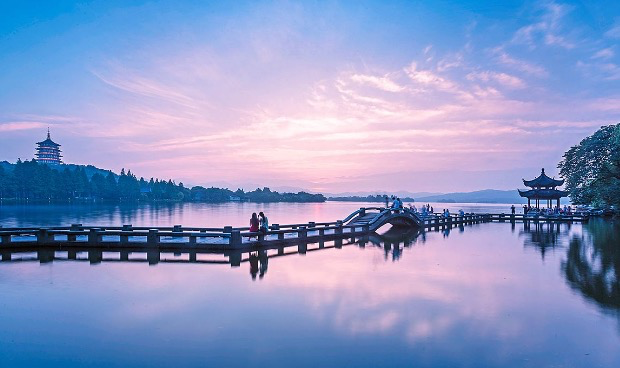
\includegraphics[width=\textwidth]{asset/03be564f-4ce8-45d1-acde-f8e0300c4e6f.png}
    \caption{一张普通的照片}
    \label{fig:img6_1}
  \end{minipage}%
  \hspace{3em}
  \begin{minipage}[h]{0.4\textwidth}
    图论里面的图, 和我们生活当中的图是一样的吗?是指我们图片、或者说我们拍照的相片、亦或是我们的地图吗?
  \end{minipage}
\end{figure}

不是的, 我给大家看一下: 

\begin{figure}[ht]
  \centering
  \begin{minipage}[h]{0.45\textwidth}
    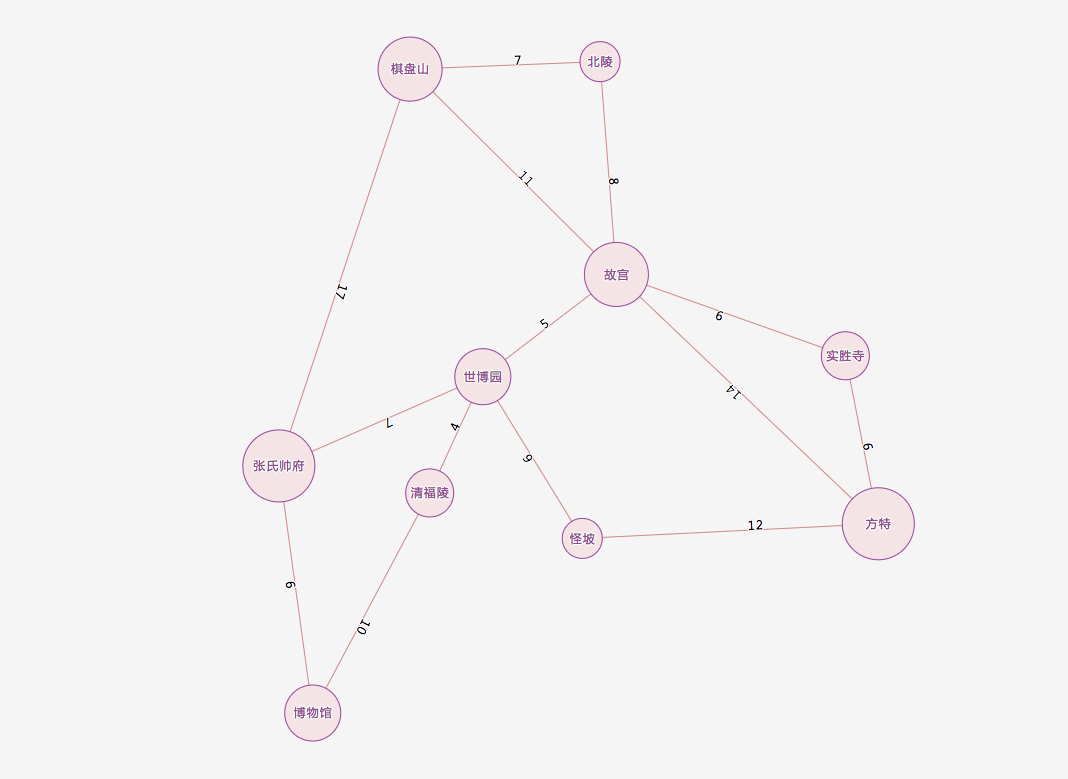
\includegraphics[width=\textwidth]{asset/54c020ae-39d8-4359-8f66-0d79cdcfc083.png}
    \caption{图论里的图}
    \label{fig:img6_2}
  \end{minipage}
  \hspace{1em}
  \begin{minipage}[h]{0.45\textwidth}
    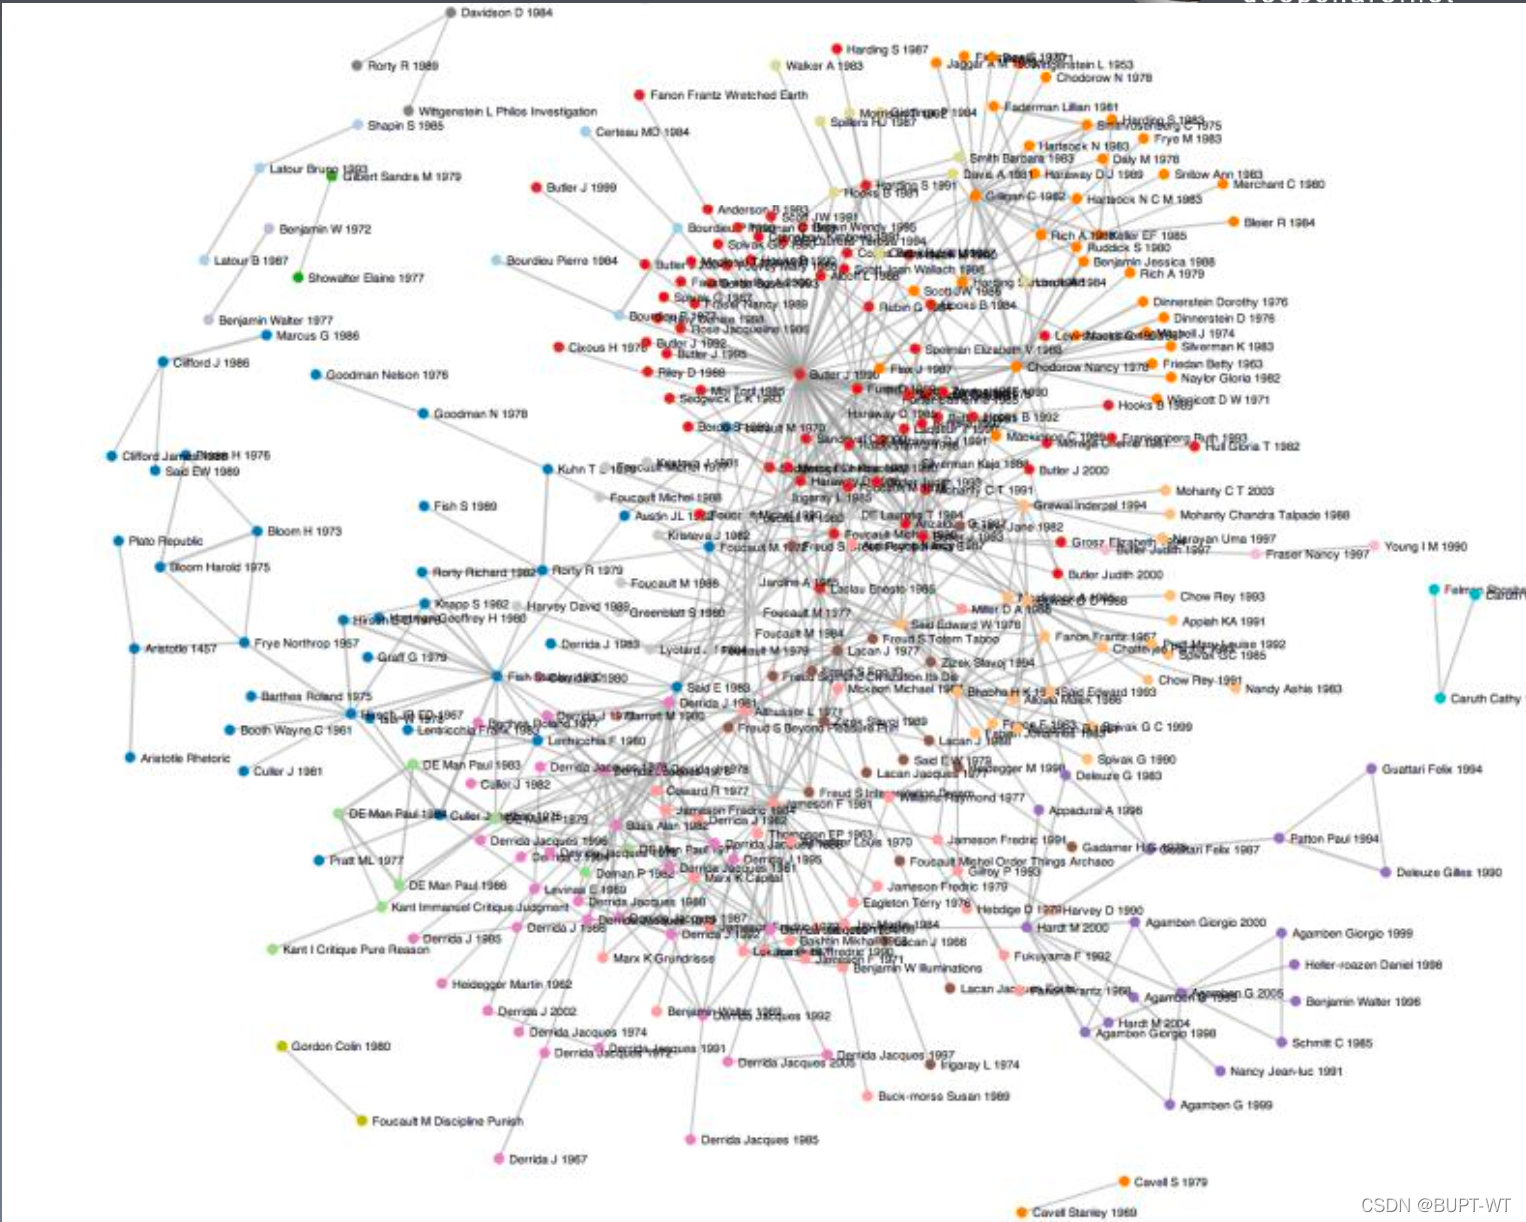
\includegraphics[width=\textwidth]{asset/2d108889-bf01-45ae-ae0c-19a3daa5a757.png}
    \caption{复杂一点的图}
    \label{fig:img6_3}
  \end{minipage}
\end{figure}

图 \ref{fig:img6_2} 就是图论里面研究的图. 它是由顶点和边构成的, 这一种网络型的结构叫做图. 当然, 复杂一点的也有, 如图 \ref{fig:img6_3}: 

所以呢, 它其实是一种抽象化的数学模型, 而不是像我们日常生活当中接触到的那样很丰富多彩, 五颜六色的. 就是一些信息量很大的点线构成网络结构. 

那为什么会有图论呢, 为什么会有人弄出这么一个很抽象的东西, 然后去去研究他呢?

图论最早的来源是柯尼斯堡七桥问题, 七桥问题我相信大家上奥数啊啥的应该都听过. 七桥问题是说, 在东普鲁士的柯尼斯堡城市里面有七座桥连接着两个小岛和河岸, 问一个人能不能从其中一个位置出发, 然后呢不重不漏的走过所有的桥, 最终回到起点, 如图 \ref{fig:img6_4}. 

\begin{figure}[ht]
  \centering
  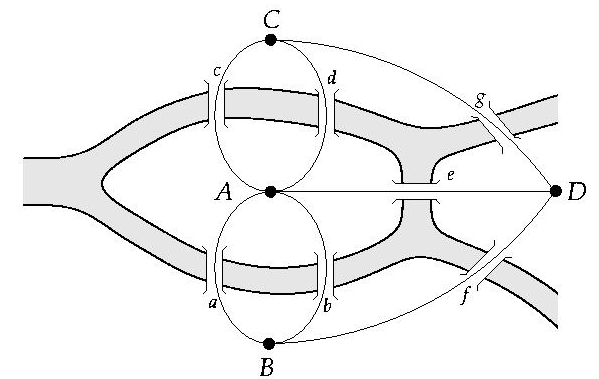
\includegraphics[width=0.7\textwidth]{asset/9d22dca2-380f-4646-8eca-179a95ce9c95.png}
  \caption{}
  \label{fig:img6_4}
\end{figure}

好多数学家, 还有数学爱好者就去研究, 就是没有人能找到走法. 后来有人把这些问题给抽象化, 用这些顶点和边来表示, 然后后来通过图论上面的方法证明出来柯尼斯堡七桥问题是无解的. 没办法从某一点不重不漏的走过任何桥然后回到顶点, 和顶点的初度入度有关了, 在这里先不展开说, 来看一下图论的概念: 

\begin{itemize}
  \item 图的构成: 顶点, 边
  \item 有向图与无向图
  \item 图的同构
  \item 边的权重
  \item 环
\end{itemize}

图的构成是什么呢?得有顶点, 有边, 顶点和边是它最基本的构成. 图还分\textit{有向图}和\textit{无向图}. 

\begin{figure}[ht]
  \centering
  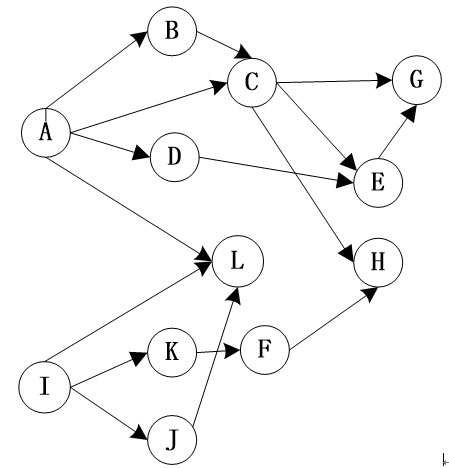
\includegraphics[width=0.5\textwidth]{asset/ee6e89d4-03e6-450b-b886-2583b91664ab.png}
  \caption{}
  \label{fig:img6_5}
\end{figure}

有向图是什么意思?就是有些边它是带方向的, 比如图\ref{fig:img6_5}中的$AD$边, 代表只能从 A 到 D, 不能从 D 到 A, 它是有向的. 而无向, 就是连接的没有箭头的边. 

图的同构是一个什么问题呢?打比方说我把 A 这一点做一个拉伸, 把 A 给拉到左边一些, 然后其他各点都保持在原地不动, 那与 A 相连的这些边是不是长度就变大了, 这样子得到一个新的图形, 和原来的图是同一个图吗? 答案是相同的图. 

所以在图论里面, 线段的长度以及顶点的大小、或者形状什么的不影响图的本质. 也就是说, 如果我们不用圆圈来表示用三角形来表示, 它还是表示同样的图. 

这就有点拓普学里面的意味了, 记得拓普学里面有个很有趣的例子: 有人问, 给你一个甜甜圈, 还给你一个碗, 还给你一个杯子. 问你杯子和碗是一类, 还是说杯子和甜甜圈是一类. 当然杯子它是一个带「把」儿的. 

就有人说, 那杯子和碗它不是挺像的吗?你把「把」儿给拿掉了, 那它不就是一样的吗?

但是按照拓普学上面的知识来说, 杯子和甜甜圈属于同一种类型, 像我们这里说的图的同构一样. 因为杯子虽然它里面是凹进去的, 但是凹进去可以再上来, 它可以进行一种揉捏的变换, 就像揉那个面团一样. 

面团可以揉下去, 也可以让他再上来对吧?做这样的变换之后会发现杯把的那个把形成的圆环其实是和甜甜圈是一样的. 甜甜圈有个环对吧?杯子的把也是有个环. 杯的深度可以通过伸缩变成一个实心的, 凹下去就没有内容的空间了. 但是形成的环, 是没办法给它去掉的. 所以, 这就是图的一个同构. 

然后我们再来说一下边的权重. 

各个边可能会有一些数值, 代表了权重. 我们在路径规划的时候, 权重可以代表什么呢?比如说 A 到 B, 这里标一个 10, 代表 A 和 B 之间, 它边的权重 10, 物理意义就是它的距离为 10 公里. 

权重可以赋予一些物理意义, 比如刚才说的路径. 最短路径的规划, 就必须对边有个权重的分配. 权重还可以表示其他的一些物理意义. 总之相当于给边赋予一个数值. 

环是什么意思呢?假设, 这里我们先不看这些箭头和这些 ABC 点, 它是不是就形成了一个闭环?在图里面它形成了一个闭环, 而这种结构就叫做就叫做环. 

主要带大家了解一下概念性的东西, 对应的图、文字描述, 如果有忘记的地方再重新看一下就行. 因为图论相对于前三个部分在人工智能里面用的场景相对比较有限. 

图论与 AI 它有什么样的关系呢?

一个就是最短路径的搜索, 边有权重之后可以根据权重值决定最短路径是怎么样的. 

还有推荐系统, 拿亚马逊或者京东打比方. 它会把你点击的这些商品用图的结构给连接在一起, 然后用图论的方式去处理, 看下一次给你推荐什么样的东西\footnote{关于推荐系统,咱们「BI 篇」里有详细的讲解,敬请期待。}. 还有包括像 Facebook、微信这种社交网络的分析, 用户与用户之间形成的结构也是图的结构. 

\hypertarget{数学如何运用于 AI}{}
\section{导论总结: 数学如何运用于 AI}

接下来我们来总结一下当前所讲的这些课. 

这几节课的总体概念都是基础, 是帮大家回忆一下相关数学知识, 或者说是帮大家了解一下. 

这些数学知识如何运用于 AI? 之前的课程中说过: 

\textbf{导数} 就是用于反向传播. 要优化损失函数必须对他进行求导, 在神经网络里面要把导数一层一层的从后往前传. 

\textbf{矩阵} 就是 AI 模型里面基本的数据结构以及参数结构. 不管是神经网络层, 还是神经网络接收的数据类型, 都是以矩阵、或者说向量的形式存在的. 

\textbf{概率统计} 应用的比较多, 在机器学习里面它也有一个统计学派叫做统计学习. 我相信大家都听说过李航的那本《统计学习方法》, 他就是以统计学的方法为一个基准点, 研究机器学习的一些方法. 里面包括一些贝叶斯分类、最大自然估计这些. 我们之后也会挑一些重点给大家讲解. 

\textbf{图论} 应用的主要是概率图的模型. 比如说大家可能听过的 BS 网络, 还有马尔科夫网络. 当然还有其他一些知识也会用于 AI, 在之后的课程会学习到. 

之后的课程里会仔细讲解 AI 中会用到的这四个知识点, 下节课我们会从导数开始, 希望让大家以最短的学习路径学到自己需要的知识, 将来能为自己的工作所用, 提高大家的\textbf{工作能力}或者\textbf{工资上限}. 